\chapter{Evaluation}\label{evaluation}

\blindtext[1]

\begin{itemize}
\tightlist
\item
  Spielbar?

  \begin{itemize}
  \tightlist
  \item
    Nur im LAN, oder auch übers Internet?
  \item
    Welche Latenz war angestrebt? Erreicht?
  \end{itemize}
\item
  WebRTC vs.~WebSockets

  \begin{itemize}
  \tightlist
  \item
    Wenn LAN-Spiel: Welchen Vorteil bringt WebRTC? (Wie viel weniger
    Latenz?)
  \end{itemize}
\item
  Emulator: emscripten-Backends vergleichen. asm.js vs.~WebAssembly.
  Emulator funktioniert mit beidem in den zu unterstützenden Browsern
  (Chrome, Firefox). Bringt es Vorteile? Bessere Framerate? Wie viel
  besser? Andere Metriken?
\end{itemize}

\section{Aufbau der Messumgebung}\label{aufbau-der-messumgebung}

\section{Ergebnisse und
Beobachtungen}\label{ergebnisse-und-beobachtungen}

https://www.sharelatex.com/learn/Pgfplots\_package

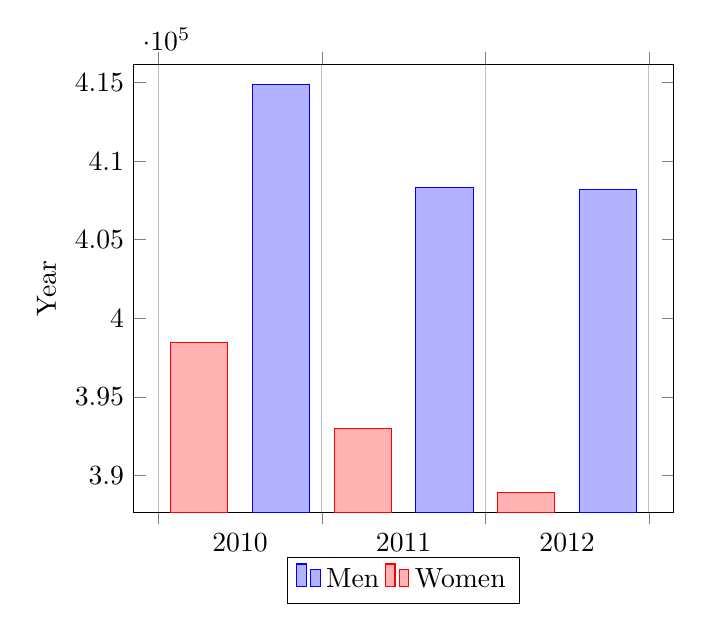
\begin{tikzpicture}
\begin{axis}[
    x tick label style={
        /pgf/number format/1000 sep=},
    ylabel=Year,
    enlargelimits=0.05,
    legend style={at={(0.5,-0.1)},
    anchor=north,legend columns=-1},
    ybar interval=0.7,
]
\addplot 
    coordinates {(2012,408184) (2011,408348)
         (2010,414870) (2009,412156)};
\addplot 
    coordinates {(2012,388950) (2011,393007) 
        (2010,398449) (2009,395972)};
\legend{Men,Women}
\end{axis}
\end{tikzpicture}

\section{Diskussion und Bewertung}\label{diskussion-und-bewertung}
